\documentclass[12pt]{article}

\usepackage[utf8]{inputenc}

\usepackage{graphicx}
\graphicspath{{img/}}

\usepackage{hyperref}
\hypersetup{
    colorlinks = true,
    linkcolor = blue,
    filecolor = magenta,
    urlcolor = cyan,
}

\newcommand{\newpar} {
    \vskip 1cm
}

\title{Investigación sobre el \texttt{malware} oculto}
\author{Noelia Díez Pinto, Cristian Camilo Morales Tapias, Ricardo Casanova, Carlos Ortega Marchamalo, Pablo Collado Soto}
\date{}

\begin{document}
    \begin{titlepage}
        \maketitle
    \end{titlepage}

    \newpage
    \tableofcontents

    \section{Introducción}
        Con el aumento del uso de las nuevas tecnologías en general y de \texttt{Internet} en particular se han incrementado los ataques e intrusiones a equipos e información. Esto puede comprometer la integridad, confidencialidad y disponibilidad de los recursos del sistema. Todo ello se debe a la creciente exposición ante ataques propiciados por un mayor conocimiento del funcionamiento de los sistemas por parte de los intrusos. Por ello están mejor preparados para encontrar y explotar vulnerabilidades. Gracias al fácil acceso y transmisión de información técnica que tenemos hoy en día, es posible incluso explotarlas desde el mismo momento en el que se da a conocer un \textit{software}. Estas son las llamadas vulnerabilidades \textit{zero-day}. Con la facilidad actual para encontrar "huecos" por los que "colarnos" en un sistema se abre la puerta a la proliferación de ataques con estrategias y tipos tremenedamente variados.

        \newpar

        A este tipo de \textit{software} cuyo objetivo es infiltrarse o dañar una computadora o un sistema de información sin el consentimiento del propietario se le conoce como 
        \texttt{malware}. Dependiendo de los efectos deseados de dicha pieza de código, el \texttt{malware} se puede clasificar en varios tipos. En el caso de nuestro grupo, nos centraremos en el \texttt{malware} oculto.

        \newpar

        Esta ocultación de \textit{software} malicioso se consigue normalmente empleando un método de \textbf{ofuscación} de su código de forma que oculta su flujo de control y su estructura quedando enmascarando su verdadera función de manera que la víctima no es consciente.

        \newpar

        Existen sistemas de detección de intrusiones o \textbf{IDS}s (\textbf{I}ntrusion \textbf{D}etection \textbf{S}ystem) que se implementan tanto en \textit{hardware} como en \textit{software} especializados en la automatización de la monitorización de redes y sistemas en busca de evidencias de violación de una determinada política de seguridad. Una adecuada elección y configuración del \textbf{IDS} puede incrementar en gran medida la seguridad de una red o sistema.

        \newpar

        A continuación ahondaremos en cada uno de los aspectos que definien al \texttt{malware} en general y al \texttt{malware} oculto en particular yendo de lo general a lo específico. Con ello esperamos haber sido concisos y explicativos en el siguiente documento. Gracias por su tiempo y atención.

    \section{¿Qué es el Malware?}
        Para poder llegar a comprender la definición de malware oculto, primero debemos analizar y entender lo que es el \texttt{malware}. La palabra malware proviene de la unión de dos palabras en inglés \textit{malicious} y \textit{software} con lo que su traducción sería programa malicioso. Es por ello que lo podemos entender el \texttt{malware} como todo tipo de software que ha sido creado con la intención de dañar cualquier sistema. El malware suele ser confundido por la mayoría de las personas con los virus, sin embargo, es importante destacar que los virus informáticos son un tipo específico de malware.

        \newpar

        El malware por lo general es creado por hackers con intenciones maliciosas. Algunas de los efectos que provocan son: dañar los dispositivos, robar datos e información personal de los usuarios, apropiarse de los recursos informáticos o negar el acceso a los mismos... Por otra parte, el objetivo de su creación está relacionado con la persona que lo diseña. Normalmente son creados para buscar algún beneficio económico, pero también han sido utilizados como una herramienta para protestas y en algunos casos incluso se ha llegado a usar como arma de guerra entre gobiernos. Destacamos que en el ámbito de la investigación se ha diseñado también malware con el objetivo de poner a prueba sistemas o de demostrar sus vulnerabilidades.

        \newpar

        En la actualidad, este tipo de programas ha encontrado en Internet el medio predilecto para poder propagarse, ya sea mediante páginas web infectadas, correo electrónico sospechoso que suele ser enviado en masa (conocido también como \textit{spam}), archivos compartidos en línea, demos de videojuegos, barras de herramientas o de cualquier otra cosa que se descargue de la red de redes. Muchas muestras relaes de malware tienen también la capacidad de autopropagarse. Una vez que se ha infectado una máquina de una red local algunos "bichos" implementan técnicas de movimeinto lateral que les permieten infectar a máquinas de la misma red. Esto supone que no existe una fuente única: cada infectado puede muchas veces contagiar. Este hecho encuentra su reflejpo en el mundo real. A pesar de lo brutal de la situación actual podemos aprender de ella y observar cómoo de fácil es que se descontrole un virus. En el caso del malware podemos llegar a experimentar escenarios parecidos como fue el caso de la \textit{Mirai Botnet} que en su punto álgido llegó a componerse de $600,000$ equipos infectados tal y como vemos en \ref{mirai_art}.

        \newpar

        En los últimos años debido a la revolución que han tenido los dispositivos móviles, estos también se han convertido en un vector de ataque importante. La evolución y el aumento del uso ilegal de estos programas maliciosos ha derivado en la necesidad, casi obligatoria, de que los usuarios utilicen alguna herramienta que sirva para combatir este software malicioso, a esta herramienta la conocemos como \texttt{antimalware}.

        \newpar

        Como hemos comentado con anterioridad existe una gran variedad de malware, y dependiendo de las características de cada uno de ellos se han clasificado en los siguientes tipos:
        
        \begin{itemize}
            \item Infeccioso
            \item Oculto
            \item Espía o \textit{spyware}
            \item Publicitario o \textit{adware}
            \item Orientados a ataques de denegación de servicio (\textit{DDoS})
            \item Secuestro de información o\textit{ransomware}
            \item Engaño 
        \end{itemize}

        \newpar

        En nuestro caso hablaremos del malware oculto, y abarcaremos desde los diferentes tipos que existen hasta su respectivo método de propagación pasando por las medidas de prevención y defensa que se deben tomar para evitar el ataque de estos programas. Pasamos pues a profundizar en aquello que define al mlaware oculto.

        \subsection{¿Y qué es el malware oculto?}
            Un malware podrá alcanzar sus objetivos siempre y cuando permanezca oculto a la vista del usuario. Es por ello que denominamos malware oculto a aquellos programas nocivos cuyo ingreso al sistema y posterior ataque ocurre de manera silenciosa, es decir, sin que el usuario lo perciba y sin su consentimiento. Dentro de esta clasificación de malware oculto podemos de igual forma encontrar diversos malwares como son:

            \begin{itemize}
                \item Troyanos
                \item \textit{Backdoors}
                \item \textit{Drive-by downloads}
                \item \textit{Rootkits}
            \end{itemize}

            \newpar

            Unas de las mejoras que han ido perfeccionando los ciberdelincuentes en los últimos años es la posibilidad de ocultar el malware, por lo que este logra permanecer por bastante tiempo en nuestro dispositivo ejecutándose en un segundo plano.

            \newpar

            Algunos lugares que han sido utilizados por estos hackers maliciosos para ocultar los malwares son:

            % TODO: Decidir que 'Accesos directos' quedarnos!

            \begin{itemize}
                \item \textbf{El registro de Windows}: Varios programas han sido creados con la posibilidad de modificar este registro para poder controlar el tiempo en el que quieran que se ejecute el software, ya sea al iniciar el sistema o después de cada tiempo programado, entre otros.
                \item \textbf{Archivos y carpetas temporales}: Es uno de los lugares donde casi siempre se oculta el malware. Ejemplos claros de estos archivos y carpetas temporales son la caché de Internet o la de datos de las aplicaciones. Al almacenarse en estos lugares una gran cantidad de información del usuario, residir ahí les permite mutar y amenzar con eliminar o difundir la información que encuentren. Con ello pueden lograr maximizar su impacto y capacidad destructiva.
                \item \textbf{Accesos directos}: Abarca las páginas web que han sido modificadas para realizar sus ataques, de igual forma pueden incluir archivos ejecutables modificados que a vista del usuario sea difícil encontrar las diferencias con respecto al original.
                \item \textbf{Accesos directos}: Muchas veces modifican o crean accesos directos de aspecto legítimo que al ser ejecutados lanzan el propio programa malicioso. Ésta similitud con los programas que un usuario espera encontrr supone una gran dificultad para su detección...
                \item \textbf{Descarga de archivos}: El malware puede entrar al sistema a través de archivos descargados, ya sean de música o simples documentos de \texttt{Word, Excel} o \texttt{PDF}. Lo mismo puede ocurrir con las aplicaciones. Todos ellos pueden ueden haber sito modificados para albergar un malware que entrará en acción tan pronto como reproduzcamos, abramos o ejecutemos alguno de estos archivos.
                \item \textbf{E-mail}: Éste es uno de los principales puntos de entrada de malware al sistema. Una forma muy popular de esparcir malware es a través de correo no deseado o \textit{SPAM}. Estos tipos de correos son un peligro inactivo hasta que el usuario por error entra en ellos y descarga algún archivo o entre en una página maliciosa. A modo de curiosidad destacamos que la palabra \textit{SPAM} deriva de un tipo de carne de consumo militar. Nunca sabes lo que puedes aprender...
            \end{itemize}

            \newpar

            El malware oculto también ha llegado al internet de las cosas o \textbf{IoT} (\textbf{I}nternet \textbf{o}f \textbf{T}hings) por en sus siglas en inglés. Este nuevo paradigma que tiende a conectar todo dispositivo a Internet ha supuesto un aumento en el número de ciberataques. Dispositivos como cámaras \texttt{IP} y lámparas inteligentes son conocidos por las medidas de seguridad tan laxas que incorporan por lo que en la actualidad pueden llegar a convertirse en los puntos débiles dentro de nuestra red. Así, este tipo de equipos pueden servir de puente para realizar ataque a nuestros ordenadores o móviles. Un caso feahaciente de ésto es la \textit{Mirai Botnet} que comentábamos antes. Tras haber infectado varias centenas de miles de quipos fue capaz de "tumbar" servicios preparados para aguantar grandes cargas de tráfico. Si bien este caso se relaciona con el malware cuyo objetivo es efectuar ataques de denengación de servicio nos muestra cómo cualquier vulnerabilidad es suficiente para que el malware pueda propagarse e infectar distintos equipos.

            \newpar

            Con todo, vamos a pasar a comentar instancias reales de este tipo de malware.

    \section{Tipos de malware oculto}
        Como hemos comentado, el mundo de los malwares es muy amplio y diverso con lo que nos encontramos muchos tipos diferentes. En nuestro caso nos centraremos en el malware oculto, que a su vez comprende muchas variantes y posibilidades. Nosotros las acotaremos centrándonos en los troyanos, las puertas traseras o \textit{backdoors}, los \textit{rootkits} y los \textit{drive-by downloads}, cuyas cualidades más reseñables comentamos más abajo.

        \subsection{Troyanos}
            Los troyanos son el primer paso de muchos ataques informáticos que se llevan a cabo. Su nombre se basa en la famosa leyenda de la mitología griega del caballo de Troya, una enorme estructura de madera que tenía el aspecto del propio animal y que, a primera vista, parecía que no entrañar ningún peligro. No obstante, en su interior albergaba a varios soldados que empleaban este procedimiento para esconderse y no ser descubiertos. Al caer la noche los soldados tomaron la hasta entonces inexpugnable ciudad de Troya.

            \newpar

            Basándose en esa idea, este tipo de malware consiste en un programa que en primera instancia parece inofensivo, hasta el punto de poder resultar atractivo, por lo que las víctimas que lo padecen no son capaces de percibir su peligrosidad debido a su apariencia amigable. Sin embargo, una vez que se descarga y llega a ejecutarse, se pone en marcha su cometido real que no es otro que el de infectar la máquina que lo aloja para posibilitar que el atacante que se encuentra detrás de él se haga con el control de la misma, todo ello de manera transparente y prácticamente imperceptible para el usuario. Estos troyanos son muchas veces el punto de partida para ataques de maypor índole. Que pueden pasar por allbergar e instalar otros tipos de malware en el equipo, por ejemplo.

            \newpar

            De este modo, en un primer momento, los troyanos se empleaban para realizar el mayor daño posible sin ningún tipo de miramiento. Intentaban desde formatear el ordenador envenenado a eliminar archivos del sistema. Sin embargo, no consiguieron la trascendencia y notoriedad que buscaban, limitados por la imposibilidad de propagarse y multiplicarse por si mismos. Ésta es una diferencia notablle con los virus y los gusanos informáticos y que les frenaba en gran medida. Por ello pasaron a buscar nuevos objetivos en los que enfocarse.

            \newpar

            Así, en la actualidad se puede llegar a lograr manejar archivos que se albergan en la máquina, copiándolos, eliminándolos o enviándolos, robar datos privados tales como números de tarjetas bancarias, controlar los procesos en ejecución, denegar el uso legítimo de servicios, obtener un registro de las pulsaciones que se producen así como de lo que se está visualizando en la pantalla. Para llevar a cabo estas acciones dependen de "terceros", esto es, programas específicos para llevar a cabo estas tareas.

            \newpar

            De forma similar, pueden también implementar diversos mecanismos que facilitan la conexión al ordenador desde otros lugares como, por ejemplo, las denominadas puertas traseras o \textit{backdoors}. Para realizar estas técnicas, los troyanos son capaces de abrir de puertos de comunicaciones o \textit{sockets} de tal forma que se consigue abrir un punto a través del que es posible alcanzar el equipo infectado.

            \newpar

            Por tanto, el cometido principal de los troyanos es ocultarse a la víctima y esconder su funcionalidad maliciosa para, a continuación, después de lograr ponerse en funcionamiento al ejecutarse el programa que lo alberga lo que posibilita acciones malvadas llevadas a cabo por él mismo o por otros sistemas o individuos a los que facilita el acceso a la máquina infectada.

            \newpar

            Este tipo de malware puede situarse en páginas que no son muy frecuentadas y que, además, resultan hasta cierto punto desconocidas, en las cuales incluso pueden encontrarse aplicaciones ejecutables que, a primera vista, no parecen entrañar ningún peligro y pueden ser, del mismo modo, de confianza y legítimas. También pueden provenir de descargas realizadas en redes \texttt{P2P} (\textit{peer-to-peer}), en las que la seguridad no es una prioridad ya que son accesibles por todo el mundo y es posible alojar archivos en ellas sin que estén sujetos a controles exhaustivos.

            \newpar

            Los troyanos se componen de dos partes de vital importania para su correcto funcionamiento e implementación. Así, constan de un cliente y un servidor, alojándose en la máquina atacada y atacante, respectivamente. Al estudiar las fases típicas de un ataque así como un ejemplo real ahondaremos más en este modelo cliente-servidor.

        \subsection{Backdoors}
            Una de las funcionalidades de las que hacen uso estos troyanos son las puertas traseras o \textit{backdoors}, por lo tanto, no constituyen un mecanismo independiente de ataque informático sino que más bien son un complemento a estos últimos.

            \newpar

            Los fines de las backdoors pueden resultar muy diversos y variados y no todos tienen por qué ser dañinos y perjudiciales. Pueden derivar de múltiples orígenes, no únicamente relacionadas a los troyanos, pues puede darse la situación de que los desarrolladores de sistemas y aplicaciones se olvidaran de eliminarlas o bloquearlas o, simplemente, continúen existiendo para efectuar determinadas tareas legales de mantenimiento o actualización de forma transparente al usuario, sin que se requiera de su participación y facilitando su experiencia y uso. Esto ocurre, por ejemplo, en equipos que reciben actualizaciones sin que su dueño sea consciente de ello. También se emplean estas \textit{backdors} para solucionar problemas técnicos mediante el acceso remoto de un especialista sin que deba mediar el usuario.

            \newpar

            En cambio, en nuestro estudio nos centraremos en aquellas que están más enfocadas a realizar acciones negativas para la víctima y que atenten contra su privacidad e intimidad.

            \newpar

            Estos recursos, tal y como su nombre bien indica, favorecen esquivar los rigurosos controles de seguridad existentes para poder acceder a un ordenador y habilitan la entrada a la máquina de forma muy sencilla y asequible, lo que simplifica que el atacante pueda obtener el mando del mismo y poner en práctica actos malintencionados y nocivos para el dueño del dispositivo. A través de esta apertura secreta se consiguen ejecutar todas las acciones perjuiciosas comentadas anteriormente.

            \newpar

            Las backdoors se originan como consecuencia de la infeccción de una máquina por parte de un troyano aunque también pueden producirse por diversos fallos de seguridad que originan ciertos resquicios que son aprovechados por los atacantes.

            \newpar

            Las puertas traseras, tal y como hemos mencionado, se implementan abriendo puertos de comunicaciones que podemos considerar "puertas" a Internet. Con ello se pueden establecer conexiones con la máquina comprometida desdde cualquier parte de la red de redes.

            \newpar

            En algunas situaciones el mecanismo de las \textit{backdoors} se empleada para crear \textit{botnets}, cuyo término proviene de la convinación de las palabras inglesas \textit{robot} y \textit{network}. No se trata de más que un conjunto de dispositivos controlados de manera remota. Es similar a un "ejército de máquinas zombies" a las que podemos ordenar tomar una serie de acciones. Los fines de este entramado se centran principalmente en generar ataques de denegación de servicio que impidan el acceso a determinadas páginas web por parte de otras personas. Para ello, hacen uso de la embergadura y capacidad del conjunto para colapsar los servidores de estos sitios efectuando un gran número de solicitudes, desencadenado el bloqueo y la caída de los mismos. Un ejemplo de ello es la \textit{Mirai botnet} que comentábamos en secciones anteriores. También se utilizan estas redes de robots para enviar masivamente los popularmente conocidos correos electrónicos basura o \textit{SPAM}, que no son más que emails con información poco relevante y que, además, pueden suponer un peligro para la seguridad de nuestros aparatos.

        \subsection{Rootkits}
            Los \textit{rootkits} son un tipo de malware que afecta al sistema operativo que se aloja en el ordenador. De este modo, logran modificar la configuración del mismo para posibilitar la presencia de mecanismos maliciosos sin que el usuario de la máquina logre percatarse de ello. Al igual que ocurre con los troyanos, no son capaces de propagarse automáticamente.

            \newpar

            Así, esta instancia es capaz de pasar desapercibida por la lista de procesos en funcionamiento e incluso por los propios antivirus. Asimismo son capaces de ocultar los archivos en los que residen y las conexiones de red que establecen con lo que son tremendamente complicados de detectar. Algunos incluso llegan a alojarse en los sectores de arranque del disco con lo que pasa a ser prácticamente imposible eliminarnos... En esos casos un formateo del disco suele ser la única solución con lo que su potencial destructivo es cuanto menos notable.

            \newpar

            Es posible, aprovechar estos accesos imperceptibles del tipo \textit{backdoor} para entrar de forma rápida y fácil al dispositivo desde el exterior y poder controlarlo para obtener información comprometida o poner en marcha acciones perversas tal y como sucede con los troyanos también.

            \newpar

            Para su instauración en un equipo se requieren permisos de escritura. El atacante, recurriendo a alguna vulnerabilidad presente en el aparato o conociendo la contraseña de un usuario con permisos puede adquirirlos. Con ello podría proceder a infectar el equipo con este tipo de malware.

            \newpar

            Distinguimos dos tipos de \textit{rootkit} según su persistencia. Por un lado, tenemos los \textit{rootkit persistentes} que se activan cada vez que se inicia todo el sistema y, por otra parte, los no persistentes, que deesaparecen tras un reinicio. Como cabría esperar el primer tipo es el más complicado de eliminar.

            \newpar

            Considerando el modelo de ejecución que implementan encontramos aquellos que se limitan al espacio de usuario mientras que otros tienen por objetivo alojarse en el núcleo del sistema operativo o \textit{kernel}. Dado que esta parte del sistema cuenta con permisos elevados y tiene acceso a todos los recursos los \textit{rootkits} que se alojan aquí tienen el potencial para desatar el caos en la máquina afectada. Para alojarse en el \textit{kernel} los \textit{rootkits} suelen modificar la imagen de éste en memoria a través del archivo \texttt{/dev/kmem} en Linux por ejemplo o hacer uso de los módulos que le podemos insertar a este mismo \textit{kernel}. Para que todo funcione este tipo de malware oculto suele alterar la tabla de llamadas al sistema para entrar en ejecución.

            \newpar

            En origen, esta actuación estaba destinada a entornos de tipo \texttt{UNIX}, de ahí su nombre pues en dicho ámbito al administrador del sistema se le denomina también como \textit{root}. Sin embargo, con el paso del tiempo buscaron un nuevo enfoque y se interesaron por máquinas equipadas con Windows en las que su comportamiento era exactamente el mismo.

            \newpar

            En cambio, no todo son conductas ilegales ya que se hallan contextos para los que sí son legítimos como, por ejemplo, la supervisión de los empleados de una empresa o corporación, la protección de datos intelectuales o frente a errores humanos como pueden ser borrados accidentales.

        \subsection{Drive-by download}
            El malware oculto de tipo \textit{drive-by download} es uno de los métodos de infeccción más simples que pueden existir. Su simplicidad radica en el hecho de que el usuario que va a ser víctica de él no debe realizar ninguna acción excepcional, pulsar en sitio alguno o aceptar ninguna descarga.

            \newpar

            El ataque se materializa cuando el individuo se adentra en una página web y, de manera inmediata y sin que muestre evidencia de ello, se inica la bajada del programa pernicioso.

            \newpar

            Para ello, en esta técnica se esconde el software nocivo de diversas formas. Por una parte, este se incluye entre el propio código \texttt{HTML} de la página web. De forma similar, puede ocurrir que se resguarde detrás de los anuncios publicitarios que aparecen en ciertos de estos sitios visitados, aprovechando determinadas carencias que puedan presentar complementos como \texttt{Java}, \textit{Flash} u otros de idénticas características. Esta es una de las razones por las que \texttt{Flash} no va a tener soporte más allá de finales de este año.

            \newpar

            En estos casos, suele suceder que el código camuflado puede constituir tan solo una pequeña parte de todo el malware en conjunto, por lo que, una vez efectuado con éxito el ataque, se solicita de forma automática el contenido restante del mismo al servidor externo que lo alberga.

            \newpar

            Las páginas web que contienen estos programas pueden ser accedidas explícitamente por el usuario al ser conocedor de ellas y realizar su busqueda en un navegador web, tal y como puede suceder con entornos de escasa seguridad relacionados con recursos un tanto peculiares como, por ejemplo, la pornografía. Un usuario también puede ser conducido a ellas a través de la recepción de correos electrónicos que le invitan a ello y ventanas emergentes. En este últimos caso, el aspecto familiar y aparentemente inofensivo favorece que la víctima en ningún momento llegue a sospechar de ellas.

            \newpar

            Conociendo ya los tipos de malware en los que se centra nuestro análisis pasamos a comentar casos de ataques reales.

    \section{Casos reales}
        Para que podamos comprender mejor el alcance que pueden llegar a tener este tipo de malware, hemos decidido recopilar información de algunos ataques reales que han sido realizados bajo la técnica del malware oculto y que han afectado a un gran número de usuarios, los cuales en algunos casos probablemente ni si quiera se han dado cuenta de haber sido comprometidos.

        \subsection{El "coronavirus" informático}
            Uno de los ataques más recientes con el uso de malware oculto está siendo el llamado \textit{"Coronavirus" informático} y es que los hackers están aprovechando la pandemia actual del \texttt{COVID-19} para ocultar malware dentro de todo tipo de documentos y vídeos. Este ataque esta siendo realizado por lo general en informaciones que nos llegan a nuestros dispositivos sobre cómo protegernos del coronavirus, los métodos de detección y actualizaciones sobre el estado de alarma. El usuario, al estar interesado en ellos, accede a abrirlos sin esperarse que estos archivos estén infectados.

            \newpar

            Según \texttt{Kaspersky}, la famosa empresa de ciberseguridad que desarrolla un antivirus homónimo, hasta la fecha han sido encontrados por los momentos $10$ archivos distintos con malware ocultos. Sin embargo, se estima de que la tendencia aumente debido es considerado un cebo perfecto, ya que es una información que se puede propagar de manera extraordinaria dentro de la población. Como podemos observar en la figura \ref{f:covid_malware} el número de dominios creados entorno al \texttt{COVID-19} ha ido aumentado de forma exponencial, es por ello que los expertos no dudan en que muchos de estos dominios terminen siendo usados por los hackers.

            \begin{figure}
                \centering
                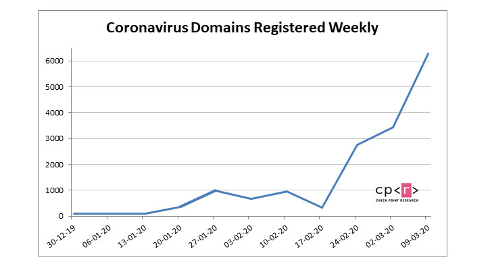
\includegraphics[width=\linewidth]{covid_malware.png}
                \caption{Dominios creadoos entorno al \texttt{COVID-19}}
                \label{f:covid_malware}
            \end{figure}

        \subsection{Aplicacones móviles ocultas}
            Según un estudio realizado por la compañía \texttt{McAfee} para el año $2019$, las aplicaciones móviles ocultas generaron aproximadamente el $50\%$ de todos los ataques a móviles de ese mismo año. El problema viene dado porque los hackers maliciosos han ido mejorando las formas de ocultar sus ataques, logrando que cada vez sean más difíciles de identificar y eliminar.

            \newpar

            Los hackers aprovechan generar versiones falsas de aplicaciones como \texttt{WhatsApp} o \texttt{Spotify} debido al alto impacto de descargas que estás pueden llegar a obtener. De igual forma se aprovechan de la popularidad de algunos juegos para engañar a los usuarios, y es que una vez el cliente haga uso de la \textit{app}, el atacante adquiere la capacidad de controlar todo el dispositivo y muchas veces el usuario ni se da cuenta de que ésto está pasando.

        \subsection{Troyano Eurograbber}
            Durante el año $2012$, en Europa se vivió bajo la acción de un troyano conocido como \texttt{Eurograbber}. Este ataque ha sido uno de los grandes asaltos informáticos ya que se saldó con la sustracción de $36$ millones de euros en toda Europa, y es que este ataque afectó cerca de unos $30.000$ usuarios de banca de países como Alemania, Italia, Países Bajos y España.

            \newpar

            En España cerca de $11.000$ personas vieron sus cuentas bancarias afectadas, lo que le permitió a los ciberdelincuentes hacerse con un botín estimado de $5,8$ millones de euros. Los ataques por lo general eran realizados a dispositivos que basados en \texttt{Android} y a los de la marca \texttt{BlackBerry} que emplean un sistema operativo propio.

        \subsection{Troyanos en diispositivos móviles}
            En el año $2019$ se descubrió la existencia de un troyano oculto en la aplicación de \texttt{Android CamScanner}, la cual cuenta con más de $100$ millones de descargas en la \texttt{Google Play Store}. Este ataque fue descubierto gracias a las investigaciones de la empresa de seguridad \texttt{Kaspersky Lab}.

            \newpar

            El ataque se realizaba mediante una biblioteca de publicidad que contenía este componente malicioso. Al descargar la aplicación y ejecutarla, los hackers ya podían acceder al dispositivo infectado y beneficiarse de la manera que quisieran, desde mostrarle publicidad intrusiva hasta robar dinero de su cuenta móvil mediante el cobro de suscripciones.

            \newpar

            Este es uno de los casos de mayor alerta debido a que se trataba de una aplicación legítima de \texttt{Android} que usaba compras integradas y a que su monetización provenía de los anuncios. La aplicación en su momento fue eliminada por \texttt{Google} de la \texttt{Play Store} para evitar que los usuarios se siguieran viendo afectados.

        \subsection{Análisis de los troyanos en los últimos años}
            Hemos analizado el informe \texttt{Ciber amenazas 2015/2016} publicado por el \texttt{Centro Criptológico Nacional} donde se muestra el análisis del aumento de dichos ataques en España. En esta gráfica podemos de igual forma observar que más de la mitad de los ataques durante el año $2015$, fueron realizados mediante troyanos. La gráfica en cuestión se adjunta en la figura \ref{f:cyber_threats}.

            \begin{figure}
                \centering
                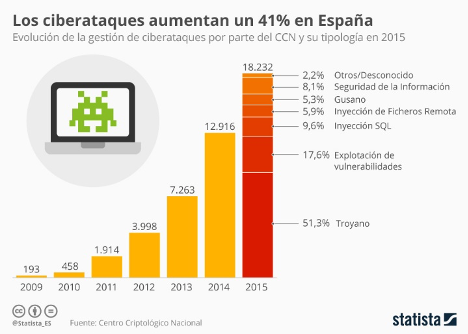
\includegraphics[width=\linewidth]{cyber_threats.png}
                \caption{Aumento de troyanos en los años 2015/2016}
                \label{f:cyber_threats}
            \end{figure}

            Otro estudio del año $2016$, realizado por la empresa \texttt{Cisco} analiza los principales ataques que recibían las empresas durante ese año, demostrando que dichos ataques no solo se relacionaban con la pérdida de dinero, sino que afectaban el prestigio y la reputación de cada compañía.

            \newpar

            En el análisis se puede apreciar que la principal vía de ataque es el uso de troyanos, ya sea tanto para pedir una recompensa por la información o que hayan sido descargados mediante softwares de manera oculta o que se hayan instalado mediante aplicaciones de Android. De igual forma se puede observar en la siguiente gráfica que otros de los principales ataques son por el uso de enlaces malignos para obtener información de los usuarios.








\end{document}